% Chapter 1

\chapter[Motivation and Background]
{Motivation and Background} % Main chapter title

\label{Chapter1} % For referencing the chapter elsewhere, use \ref{Chapter1} 

%----------------------------------------------------------------------------------------






% Define some commands to keep the formatting separated from the content 
\newcommand{\keyword}[1]{\textbf{#1}}
\newcommand{\tabhead}[1]{\textbf{#1}}
\newcommand{\code}[1]{\texttt{#1}}
\newcommand{\file}[1]{\texttt{\bfseries#1}}
\newcommand{\option}[1]{\texttt{\itshape#1}}

%----------------------------------------------------------------------------------------

\section[Quantum info processing and Qubit candidates]{Quantum info processing and Qubit candidates}

The bit is the basic unit of information in computing and digital communications. A bit can have one value, which can be 1 or 0, that represents the logical states in a 2-level logic system. In modern digital computers, these two states exits as low and high voltages in highly integrated circuits. Just like bit for classical computing, qubit is the basic unit of information in QIP, which encodes 1 and 0 into 2 distinguishable quantum states. As the qubits behaves in the manner of quantum mechanism, it gives rise to the phonomena of superposition and entanglement, which enables the processing of massive number of calculations. Previous difficult tasks in classical computing such as simulation of quantum systems or factoring of numbers will be finished quick and efficiently by quantum computers.

For the realisation of quantum computer,  the first priority is to find a fitting candidate as qubit. Five principles have been brought up for the candidates choosing by [Journal,name]:

1. A scalable physical system with well characterized qubits

2. The ability to initialize the state of qubits to a simple fiducial state

3. Long relevant decoherence times, much longer than gate operation time

4. A "universal" set of quantum gates

5. A qubit-specific measurement capability

Color centers are optically active impurities that are responsible for the colors in crystal that are transparent due to large band gap. Color centers are atom-like solid systems, with appropriate electronic structure and symmetry in crystal, they are the candidates for qubits. Additionally, it is practical to require a long enough coherent time for the operation regarding QIP.

Lots of research works has been done with NV$^{-}$, which has excellent spin properities at ambitent condition, it has also been proved that it is possible to execute an all optical access to its spin.[reference from all optical paper]. Yet due to the transform of symmetry during the excitation process, NV$^{-}$ has a big phonon side band following the ZPL. Moreover, the C3v symmetry leaves the color centre vulnerable towards the environment electric field, resulting in spectral diffusion, which is caused by the flipping of charging state. These disadvantages has reduced the generation rate of coherent photon generation rates and limit the development of NV-quantum networks[Lachlan paper].
%----------------------------------------------------------------------------------------

\section[Silicon vacancy as a Qubit candidate]{Silicon vacancy as a Qubit candidate}

SiV is considered as the next promising qubit candidate after NV. It has irresistibly excellent optical properties, and is also possible to achieve an all optical intiallizaiton, read out and coherent preparation.

SiV$^{-}$ has a D$_{3d}$ symmetry with the symmetry axis along the <111> crystal direction. The color center consists of a substitial Silicon atom and a carbon vacancy. Due to the size difference between Silicon atoms and carbon atoms, it is expected that the Silicon atom will sit between 2 lattice site instead of on a lattice site[Goss etal,  Gali and Maze, ]. The inversed symmetry offers SiV$^{-}$ extra shield from the environment small electric field.

Experimentally it is observed that the SiV$^{-}$ has outstanding optical properties, 70$\%$ of its fluorescence couples into a sharp ZPL of 1.68eV. At cryogenic temperature this ZPL can be resolved with a fine structure of 4 lines. These four lines are signed to the electronic transitions between the ground state and the first excited state of SiV$^{-}$. Theoretical calculation based on the group theory and ab initio method offers us a model of the SiV$^{-}$ electronic structure with a ground state of 2 folded degeneracy and even parity, a first excited state of 2 folded degeneracy of uneven parity and a second excited state of none degeneracy with even parity.[Goss etal] This calculation fits the observation as only the electronic transition between levels of different parity is allowed, due to the -1 parity of photons, thus only the 4 transitions between the first excited state and the ground state would be allowed, as signed to the 4 line structure of ZPL. Since this is a E to E transition, no dramatic symmetry change has been involved, less phonon would be involved in the relaxation, which fits the observation of the sharp ZPL with small phonon side band. 

Lachlan et al showed the probility to read out and coherently prepare electronic spin in individual SiV$^{-}$ centers via resonance excitation. The SiV$^{-}$ was first initialized by resonantly pumping the spin-flipping transition that is weakly allowed due to the off axis residue of the magnetic field.








\FloatBarrier
\begin{figure}[h]
\centering
\includegraphics[width=0.7\linewidth]{Figures/pic/WP_20160921_20_40_25_Pro_LI}
\caption{}
\label{fig:wp20160921204025proli}
\end{figure}
\FloatBarrier

\begin{figure}[h]
\centering
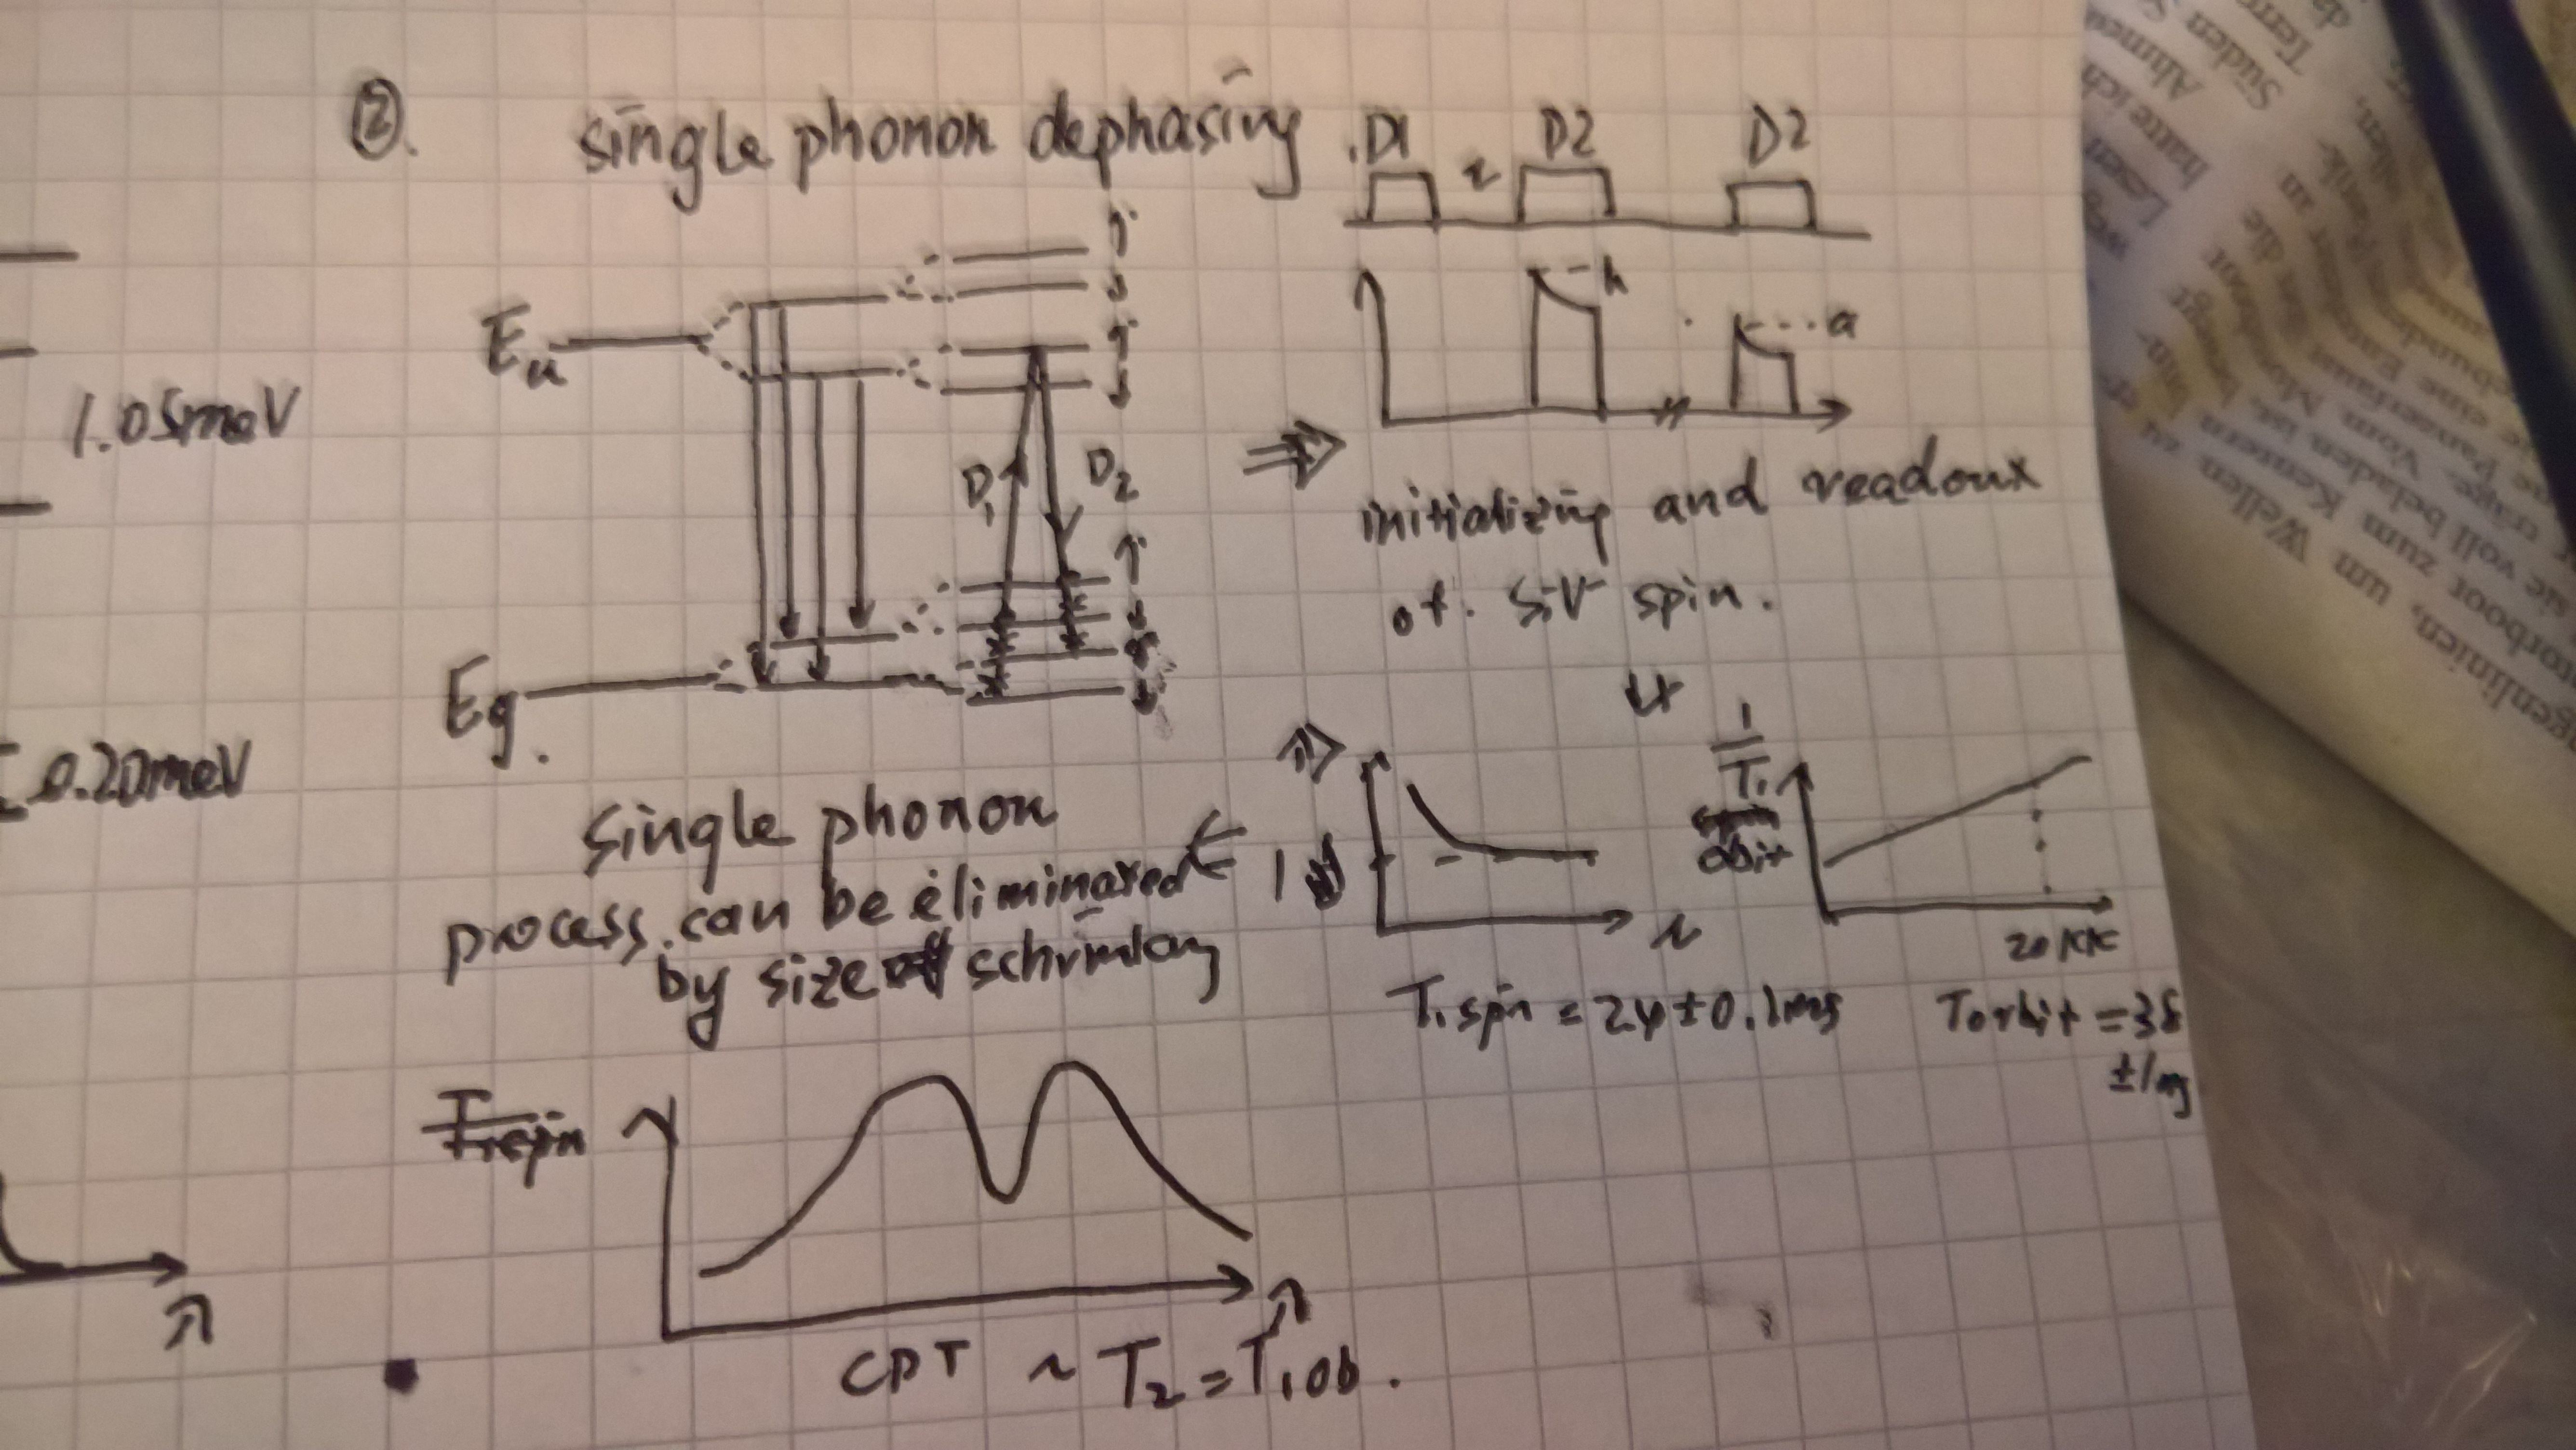
\includegraphics[width=0.7\linewidth]{Figures/pic/WP_20160921_20_40_32_Pro_LI}
\caption{}
\label{fig:wp20160921204032proli}
\end{figure}
\FloatBarrier

%----------------------------------------------------------------------------------------

\section[Silicon vacancies in nanodiamonds]{Silicon vacancies in nanodiamonds}
\FloatBarrier
\begin{figure}[h]
\centering
\includegraphics[width=0.7\linewidth]{Figures/pic/WP_20160921_20_40_48_Pro_LI}
\caption{}
\label{fig:wp20160921204048proli}
\end{figure}
\FloatBarrier

\paragraph{Band-bending near the surface of diamond}  


%--------------------------------------------------------------------------------------

\section[Motivation of the thesis, unsolved problem]{Motivation of the thesis, unsolved problem}
\FloatBarrier
\begin{figure}[h]
	\centering
	\includegraphics[width=0.7\linewidth]{Figures/pic/WP_20160921_20_40_42_Pro_LI}
	\caption{}
	\label{fig:wp20160921204042proli}
\end{figure}
\FloatBarrier
